\begin{frame}{introduction}{chain of musical communication}
      \vspace{-3mm}
        \begin{figure}
                \centering
                \begin{picture}(140,35)
                    %boxes
                    %\only<1>{\color{gtgold}
                    {\put(0,30){\ovalbox{\footnotesize{\parbox{20mm}{\vspace{2mm}\centering{\only<1>{\textcolor{gtgold}}{composition}}}}}}}
                    %}
                    \put(30,30){\ovalbox{\footnotesize{\parbox{20mm}{\vspace{2mm}\centering{\only<2>{\textcolor{gtgold}}{performance}}}}}}
                    \put(60,30){\ovalbox{\footnotesize{\parbox{20mm}{\vspace{2mm}\centering{\only<3>{\textcolor{gtgold}}{production}}}}}}
                    \put(90,30){\ovalbox{\footnotesize{\parbox{20mm}{\vspace{2mm}\centering{\only<4>{\textcolor{gtgold}}{distribution}}}}}}
                    \put(120,30){\ovalbox{\footnotesize{\parbox{20mm}{\vspace{2mm}\centering{\only<4>{\textcolor{gtgold}}{consumption}}}}}}
        
                    % horizontal
                    \put(22.4,30.6){\vector(1,0){7.8}}
                    \put(52.4,30.6){\vector(1,0){7.8}}
                    \put(82.4,30.6){\vector(1,0){7.8}}
                    \put(112.4,30.6){\vector(1,0){7.8}}
                \end{picture}
            \end{figure}
            \vspace{-27mm}
    \begin{itemize}
        \item<1-> \textbf{creation of musical ideas} (``score'')
            \begin{itemize}
                \item   defines style and idea
            \end{itemize}
        \smallskip
        \item<2-> \textbf{realization of musical ideas} into acoustical rendition 
            \begin{itemize}
                \item   interpretation, modification, addition, and dismissal of score information
                \item   unique acoustic representation of score
            \end{itemize}
        \smallskip
        \item<3-> \textbf{recording, mixing, and editing} (in case of record media)
            \begin{itemize}
                \item   editing and splicing of recorded data; timbre, equalization choices
                \item   not separable from performance in a recording
            \end{itemize}
        \smallskip
        \item<4-> \textbf{distribution \& listening}
            \begin{itemize}
                \item   music recommendation and discovery
            \end{itemize}
    \end{itemize}
    \inserticon{direction}
\end{frame}
\begin{frame}{introduction}{musical communication and AI}
      \vspace{-3mm}
        \begin{figure}
                \centering
                \begin{picture}(140,35)
                    %boxes
                    %\only<1>{\color{gtgold}
                    {\put(0,30){\ovalbox{\footnotesize{\parbox{20mm}{\vspace{2mm}\centering{\only<1>{\textcolor{gtgold}}{composition}}}}}}}
                    %}
                    \put(30,30){\ovalbox{\footnotesize{\parbox{20mm}{\vspace{2mm}\centering{\only<2>{\textcolor{gtgold}}{performance}}}}}}
                    \put(60,30){\ovalbox{\footnotesize{\parbox{20mm}{\vspace{2mm}\centering{\only<3>{\textcolor{gtgold}}{production}}}}}}
                    \put(90,30){\ovalbox{\footnotesize{\parbox{20mm}{\vspace{2mm}\centering{\only<4>{\textcolor{gtgold}}{distribution}}}}}}
                    \put(120,30){\ovalbox{\footnotesize{\parbox{20mm}{\vspace{2mm}\centering{\only<5>{\textcolor{gtgold}}{consumption}}}}}}
        
                    % horizontal
                    \put(22.4,30.6){\vector(1,0){7.8}}
                    \put(52.4,30.6){\vector(1,0){7.8}}
                    \put(82.4,30.6){\vector(1,0){7.8}}
                    \put(112.4,30.6){\vector(1,0){7.8}}
                \end{picture}
            \end{figure}
            \vspace{-27mm}
\vspace{-5mm}
\begin{columns}
    \column{.7\linewidth}
    %\begin{itemize}
        %\item[]   AI can advance all links of the musical communication chain:
        \begin{itemize}
        \item<1->   {\textbf{composition}}
            \begin{itemize}
                \item   intelligent assistance, e.g., ideas, auto-arrangements 
                \item   automatic composition 
            \end{itemize}
        \item<2->   {\textbf{performance}}
            \begin{itemize}
                \item   interactive music education systems
                %\item   enable new ways of controlling sound
                %\item   interact with artificial performers
                \item   generation of 'human' performance
            \end{itemize}
        \item<3->   \textbf{production}
            \begin{itemize}
                %\item   parametrize and suggest
                \item   auto-edit and auto-mix
            \end{itemize}
        \item<4->   \textbf{distribution}
            \begin{itemize}
                \item   match music style and consumer
            \end{itemize}
        \item<5->   \textbf{consumption}
            \begin{itemize}
                \item   intelligent music discovery \& adaptable music
            \end{itemize}
            \end{itemize}
    %\end{itemize}
    \column{.3\linewidth}
        \only<1-2>{\begin{itemize}
            \only<1>{\item example:\\ DeepBach \includevideo{DeepBach.mp4}}
            \only<2>{\item example:\\ Hatsune Miku \includevideo{HatsuneMiku.mp4}\\ Shimon \includevideo{shimon.mp4}}
        \end{itemize}}
        \only<1>{%\bigskip\bigskip\bigskip
            \begin{figure}
                \vspace{13mm}
                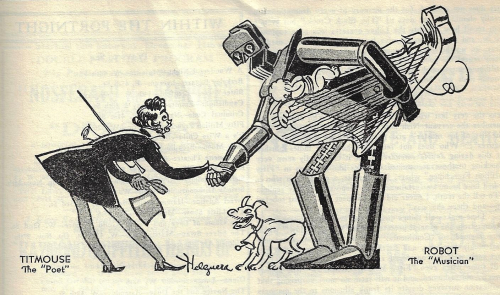
\includegraphics[scale=.7]{graph/musical-robots}
            \end{figure}
            \addreference{\href{https://longstreet.typepad.com/thesciencebookstore/2017/06/the-invasion-of-musical-robots-1929.html}{longstreet.typepad.com/thesciencebookstore/2017/06/the-invasion-of-musical-robots-1929.html}}}
        \only<2>{%\bigskip\bigskip\bigskip
            \begin{figure}
                \vspace{10mm}
                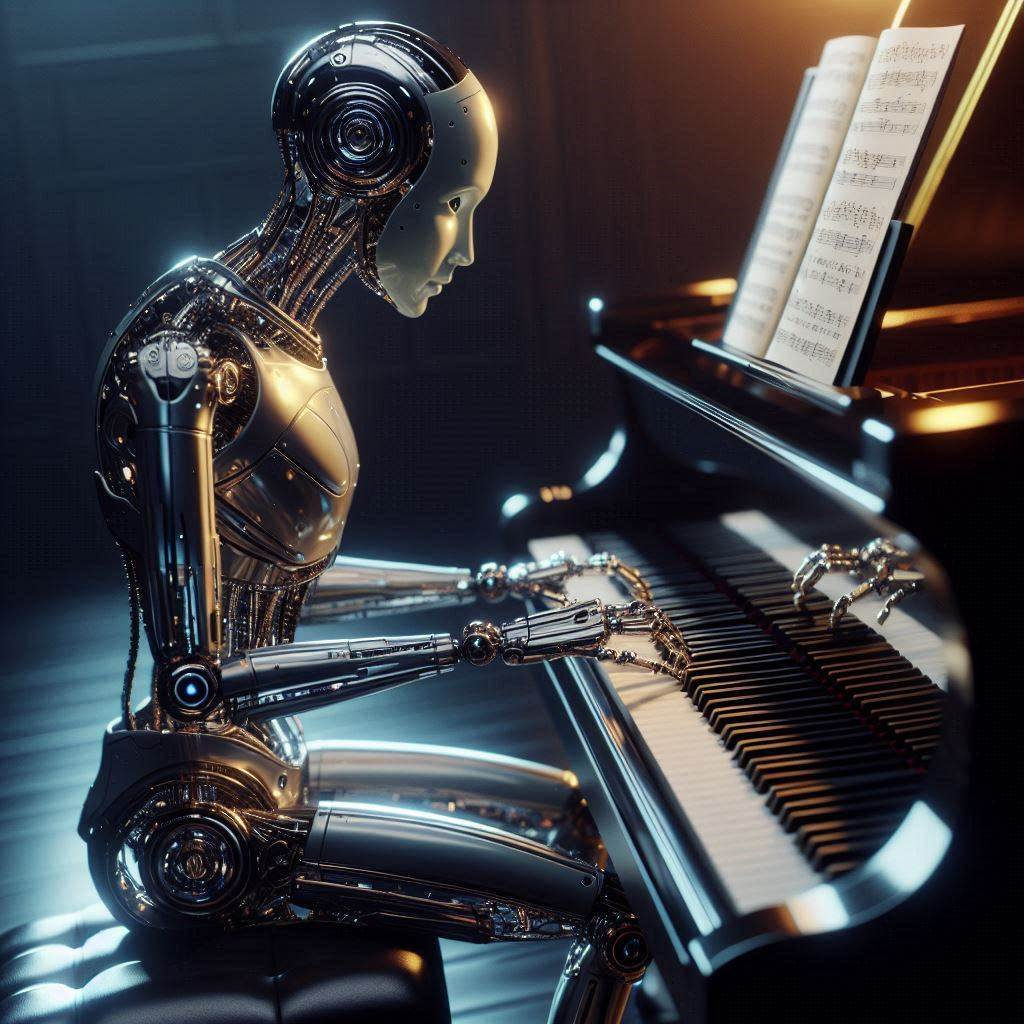
\includegraphics[width=.8\columnwidth]{ai-performer}
            \end{figure}}
        \only<4->{%\bigskip\bigskip\bigskip
            \begin{figure}
                \vspace{20mm}
                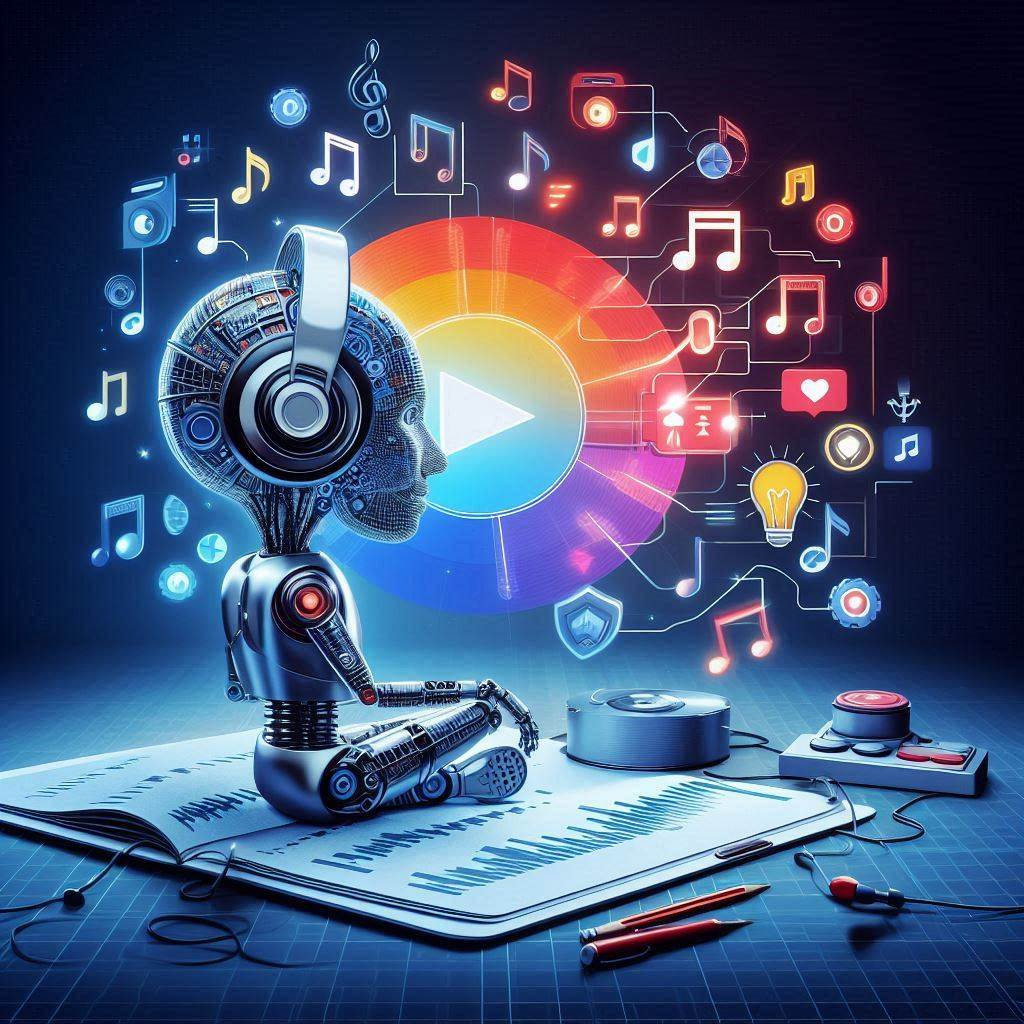
\includegraphics[width=.8\columnwidth]{ai-music-discovery}
            \end{figure}}
    \end{columns}
\end{frame}
